\section{Der Algorithmus von Berlekamp}
\label{sec:berlekamp}
Sei im Folgenden $\F_q$ ein endlicher Körper von Charakteristik $p$ und
$f(X) \in \F_q[X]$ monisch. Ziel dieses Abschnittes ist ein Algorithmus, der eine
vollständige Faktorisierung von $f(X)$ über $\F_q$ angibt.

\subsection{Idee}
Die grundlegende Idee des Berlekamp-Algorithmus besteht in folgendem Lemma.

\begin{lemma}\label{lemma:berlekamp1}
  Es gilt
  \[ X^q - X = \prod_{a\in \F_q} (X- a) \in \F_q[X] \,.\]
\end{lemma}
\begin{proof}
 \autocite[Theorem 6.1 mit Corollary 4.5]{wan2003lectures}.
\end{proof}

Ersetzen wir $X$ durch ein Polynom $g(X) \in \F_q[X]$, so erhalten wir 
\[ g(X)^q - g(X) = \prod_{a\in \F_q} (g(X) - a)\]
und können uns nun überlegen, falls wir ein Polynom $g(X)$ mit
$g(X)^q - g(X) \bmod f(X)$ haben, dann 
\[ f(X) \mid \prod_{a\in \F_q} (g(X)-a) \,,\]
was zumindest eine teilweise Faktorisierung von $f(X)$ liefern könnte.

Dass dies in der Tat funktioniert, zeigt nachstehender Satz, der obige
Idee zusammenfasst und konkretisiert.

%\begin{lemma}
  %Sei $g(X) \in \F_q[X]$. Dann ist äquivalent:
  %\begin{enumerate}
    %\item $g(X)^q \equiv g(X) \bmod f(X)$
    %\item $f(X) \mid \prod_{a \in \F_q} (g(X) -a)$
    %\item $f(X) \mid \prod_{a\in \F_q} \ggT(f(X), g(X)-a)$
  %\end{enumerate}
%\end{lemma}
%\begin{proof}
  %\autocite[Lemma 9.3]{wan2003lectures}.
%\end{proof}

\begin{thm}
  \label{satz:berlekamp1}
  Sei $g(X) \in \F_q[X]$ mit 
  \[ g(X)^q \equiv g(X)  \bmod f(X)\,,\]
  so gilt
  \[ f(X) = \prod_{a\in \F_q} \ggT(f(X),g(X)-a)\]
  und die $\ggT$s sind paarweise teilerfremd.
\end{thm}
\begin{proof}
  \autocite[Theorem 9.1]{wan2003lectures}.
\end{proof}


\subsection{Die Berlekamp-Algebra}

Damit haben wir nun eine Motivation für folgende Definition.

\begin{definition}
  Der \emph{Berlekamp-Raum zu $f(X)$} bzw. die \emph{Berlekamp-Algebra zu
  $f(X)$} ist
  \[ \cB_f := \{ h(X) \in \F_q[X]:\ \deg h < \deg f, h(X)^q \equiv h(X) \bmod
    f(X)\}\,.\]
\end{definition}

\begin{bemerkung}
  In der Tat wird $\cB_f$ offenbar zu einer $\F_q[X]\big/(f(X))$-Algebra.
\end{bemerkung}

Nun können wir ein wesentliches Resultat zitieren:

\begin{thm}
  \label{satz:berlekamp2}
  Es gilt:
  \[ \dim_F(\cB_f) = s\,,\]
  wobei $s$ die Anzahl irreduzibler paarweise verschiedener Faktoren von $f(X)$
  ist.
\end{thm}
\begin{proof}
  \autocite[Satz 6.2]{hach2013ek}.
\end{proof}

Nun stellt sich natürlich die Frage, wie man konkret Elemente aus der
Berlekamp-Algebra zu $f(X)$ findet. Blickt man noch einmal auf die Definition
von $\cB_f$, so erkennt man, dass $\cB_f$ gerade der Kern folgender linearen
Abbildung ist:
\[ \Gamma_f:\ \funcdef{
  \F_q[X]_{<\deg f} &\to& \F_q[X]_{<\deg f},\\
  g(X) &\mapsto& g(X)^q - g(X) \bmod f(X)\,.}\]
Nun können wir aber eine Darstellungsmatrix von $\Gamma_f$ angeben, da wir
simplerweise eine Basis von $\F_q[X]_{<\deg f}$ angeben können durch
\[ \{ 1, X, X^2, \ldots, X^{\deg f -1}\}\,. \]

\subsection{Der Berlekamp-Algorithmus}

Eine Kleinigkeit fehlt obigem Vorgehen noch, um daraus sicher eine teilweise
Faktorisierung von $f(X)$ gewinnen zu können. Es ist a priori nicht klar, dass
in \thref{satz:berlekamp1} die auftretenden $\ggT$s eine echte, also nicht
degenerierte, Faktorisierung von $f(X)$ liefern. Doch dies ist offensichtlich,
falls $g(X) \in \cB_f \setminus \F_q$ gewählt wird. Dann ist $\deg g < \deg f$
und daher $\ggT(f(X),g(X)-a) \neq f(X)$ für alle $a \in \F_q$.

Letztlich liefert noch nachstehendes Lemma die Grundlage für eine rekursive
Anwendung des Algorithmus:

\begin{lemma}
  \label{lemma:berlekamp3}
  Ist $a(X)\in \F_q[X]$ monisch mit $a(X) \mid f(X)$, so ist
  \[ \pi: \funcdef{ \cB_f &\to& \cB_a \\ g(X) &\mapsto& g(X) \bmod a(X)} \]
  eine surjektive lineare Abbildung.
\end{lemma}
\begin{proof}
  klar.
\end{proof}

\begin{comment}
  Ist $\pi$ nicht sogar ein $\F_q[X]/(a(X))$-Algebrenhomomorphismus??
\end{comment}


\subsubsection{Implementierung}
Um tatsächlich eine \emph{vollständige} Faktorisierung zu erhalten, muss man 
sich noch überlegen, dass dies mit Hilfe des Berlekamp-Algorithmus nur möglich 
ist, falls $f(X)$ quadratfrei ist (vgl. \thref{satz:berlekamp2}!). Daher sei 
im Folgenden $f(X)$ stets ein quadratfreies, monisches Polynom über $\F_q[X]$.

\paragraph{Berechnung einer Basis von $\cB_f$} Die Basis des Berlekampraumes
berechnen wir mit den in \autoref{sec:linalg} vorgestellten Methoden der
linearen Algebra.

\haskellinput{Algorithmen/Berlekamp}{berlekampBasis}

Die Funktion ħred iħ liefert dabei gerade das ħiħ-te Basiselement der
kanonischen Basis von $\F_q[X]\big/(f(X))$.

\paragraph{Der Berlekamp-Algorithmus} Bei einer konkreten Umsetzung des
Berlekamp-Algorithmus bleibt immer die Frage, wie ein Element $g(X)\in
\cB_f\setminus \F_q$ zu wählen ist. Wir haben uns entschieden, stets das zweite
Basiselement (das erste ist immer $1$) zu wählen. Sicherlich könnte man auch
ein zufälliges Element wählen; dies widerspricht aber der Funktionalität 
von Haskell.

\haskellinput{Algorithmen/Berlekamp}{berlekampFactor}

Die Berechnung der neuen Basis bei der rekursiven Anwendung ist aufgrund
\thref{lemma:berlekamp3} relativ einfach, da $\pi$ simplerweise auf die schon
vorhandene Berlekampbasis angewendet werden kann.

\begin{beispiel}
  Angenommen wir wollen das Polynom 
  \[ X^5 + X^4 + 3 X^3 + 3 X^2 + 2 X + 2 \ \in \F_5[X]\]
  faktorisieren. Wir berechnen also
  \[ \begin{array}{r@{\ \equiv\ }l@{\ \bmod f(X)}}
    1^5 & 1\\
    X^5 & 4X^4 + 2X^3 + 2 X^2+ 3X + 3\\
    X^{10} & X^2\\
    X^{15} & 2X^4 + 2X^3 + X^2 + X + 4\\
    X^{20} & X^4
  \end{array} \]
  und erhalten damit eine Darstellungsmatrix von $\Gamma$ bezüglich der Basis 
  $\{ 1, X, X^2, X^3, X^4\}$ von $\F_5[X]_{<5}$ und können diese in
  Zeilenstufenform bringen:
  \[ D_\Gamma = \begin{bmatrix}
      1& 0& 0& 0& 0\\ 
      3& 3& 2& 2& 4\\ 
      0& 0& 1& 0& 0\\ 
      4& 1& 1& 2& 2\\ 
      0& 0& 0& 0& 1\end{bmatrix} \sim 
      \begin{bmatrix}
      1& 0& 0& 0& 0\\ 
      0& 1& 0& 3& 0\\ 
      0& 0& 1& 0& 0\\ 
      0& 0& 0& 0& 1\\
      0& 0& 0& 0& 0\end{bmatrix}\,. \]
  Also ist eine Basis von $\cB_f$ gegeben durch
  \[ B_f := \{ 1, X^3 +X, X^2, X^4\}\,.\]
  Wir wählen -- wie oben beschrieben -- das zweite Basiselement $h(X) = X^3 +X$
  aus und berechnen
  \[ \begin{array}{r|lllll}
      a\in \F_q & 0 & 1 & 2 & 3 & 4 \\\hline
      \ggT(f(X), h(X)-a) & X^2+2 & X^2+4X+3 & 1 & 1 & X+2\end{array}\,.\]
  Dies erlaubt nun iterative Anwendung des Berlekamp-Algorithmus, nämlich für 
  $X^2+2$, $X^2+4X+3$ und für $X+2$. Letzteres ist natürlich offensichtlich 
  irreduzibel.

  Für $f_1(X) := X^2+2$ haben wir 
  \[ B_f \bmod f_1(X) = \{ 1, 0, 3, 4\}\]
  und für $f_2(X) := X^2+4X+3$
  \[ B_f \bmod f_2(X) = \{1,1,X+2,1\}\,.\]
  Für $f_1$ bricht der Berlekamp-Algorithmus sofort ab, da offenbar die
  Dimension des Berlekampraumes $1$ ist.
  Für $f_2$ wählen wir $h(X) = X+2$ und erhalten 
  \[ \begin{array}{r|lllll}
      a\in \F_q & 0 & 1 & 2 & 3 & 4 \\\hline
      \ggT(f_2(X), h(X)-a) & 1 & 1 & X+3 & 1 & X+1\end{array}\,.\]
  Damit ist die vollständige Faktorisierung von $f(X)$ über $\F_5$ bekannt:
  \[ f(X) = (X+1)(X+2)(X+3)(X^2+2)\,.\]
\end{beispiel}


\subsection{Alternative Implementierungen}

Es ist offensichtlich, dass man verschiedene Wahlen hat, den rekursiven Aufruf
des Berlekamp-Algorithmus zu gestalten. Die zweite Möglichkeit, die wir
implementiert haben und hier aufzeigen möchten, besteht darin, lediglich auf
den ersten nicht-trivialen $\ggT$ zu warten und in zwei rekursiven Aufrufen mit
eben jenem $\ggT$ und seinem Kofaktor in $f(X)$ zu enden.

\haskellinput{Algorithmen/Berlekamp}{berlekampFactor2}

\subsubsection{Ein kleiner Vergleich}

Es hat sich herausgestellt, dass beide Varianten nahzu identische Laufzeiten
haben. Bei einem kleinen Vergleich von je 30 Polynomen eines Grades
stellt sich heraus, dass letztere Variante in kleinen Graden schneller ist,
wohingegen die erste Variante in höheren Graden effizienter arbeitet.
\autoref{fig:berlekamp} fasst die Ergebnisse zusammen.

\begin{figure}
  \caption{Vergleich der Berlekamp-Varianten über $\F_5$ und $\F_{5^3}$}
  \label{fig:berlekamp}
  \centering
  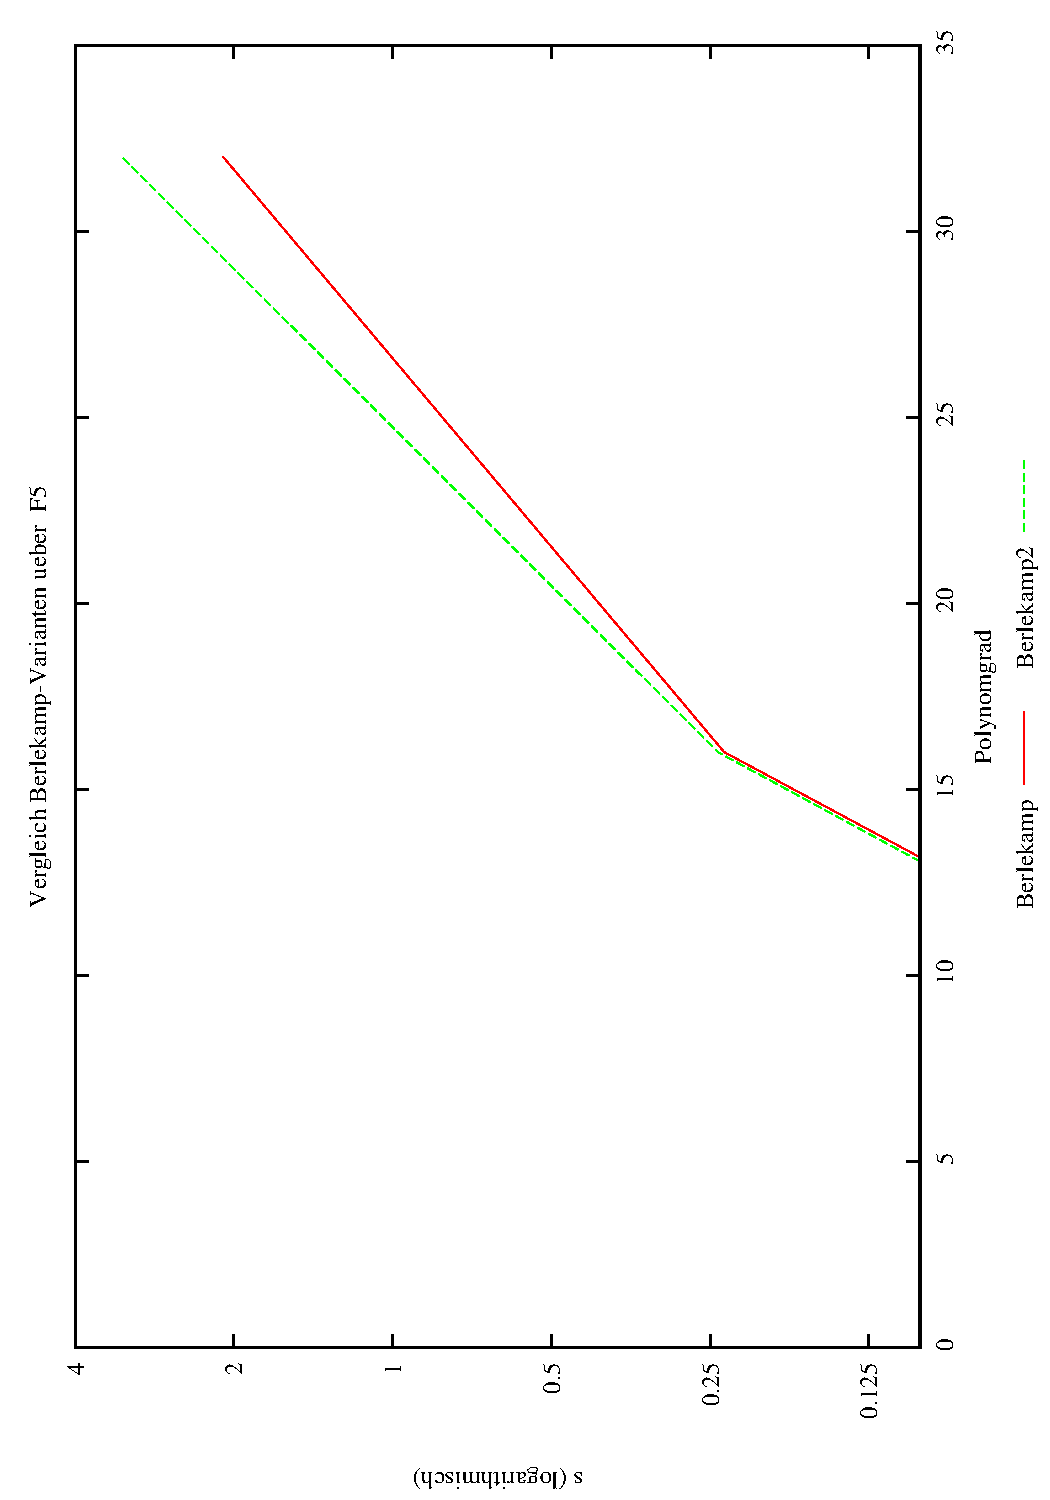
\includegraphics[width=0.7\textwidth,angle=-90]{plots/benchBerle_F5.pdf}
  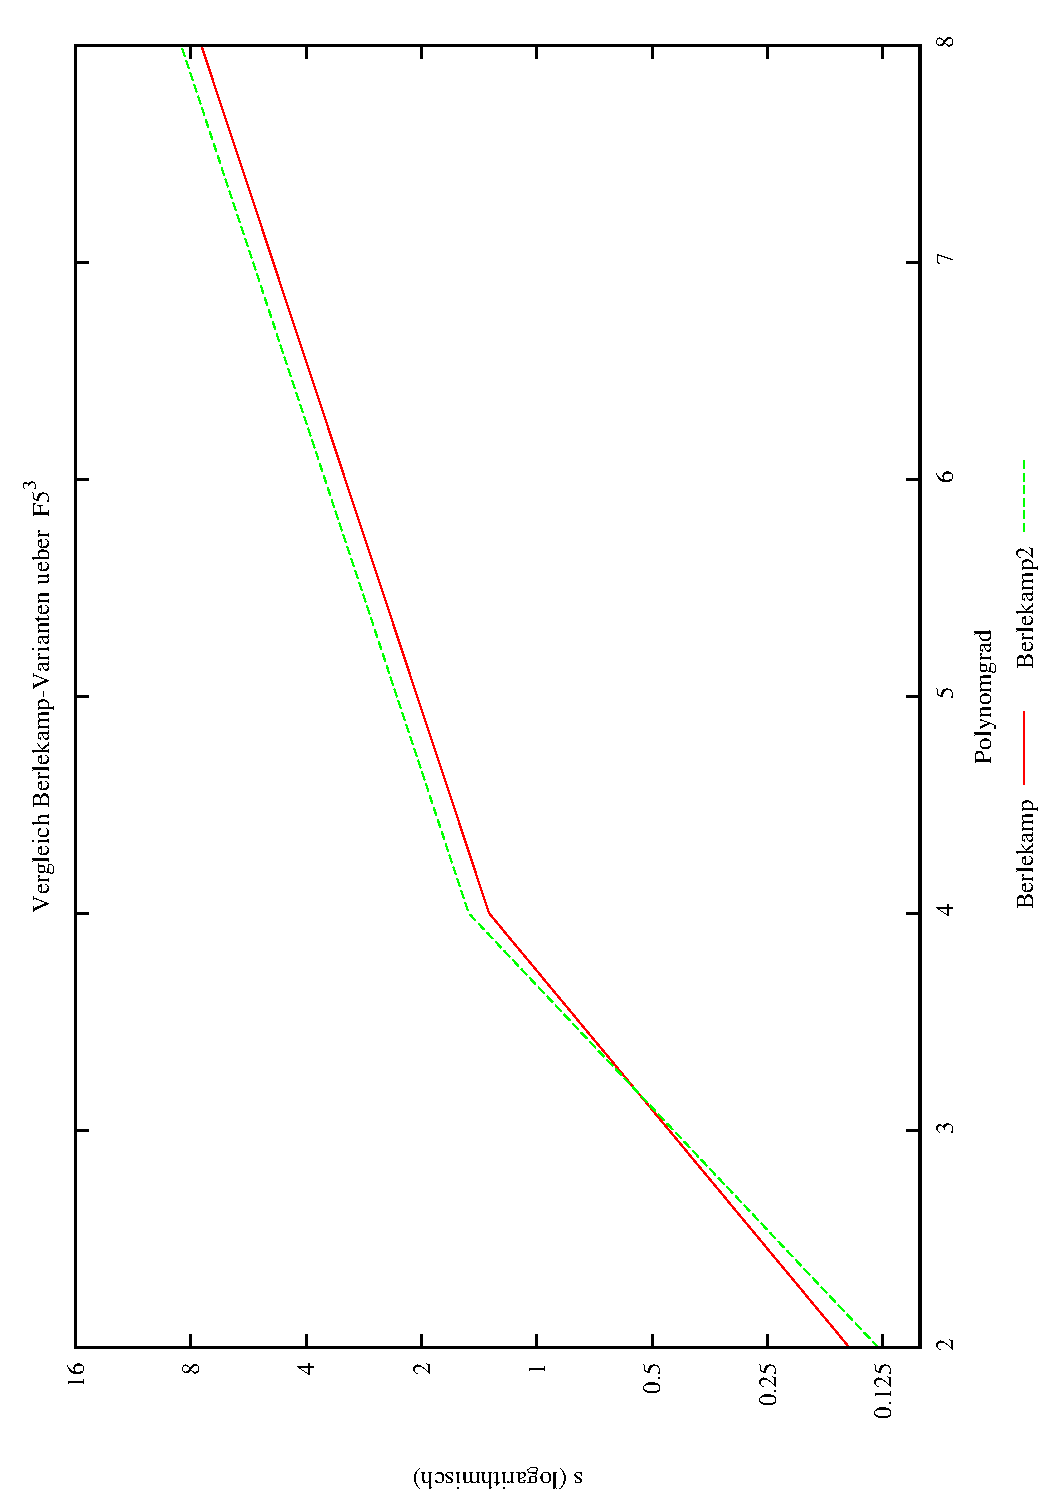
\includegraphics[width=0.7\textwidth,angle=-90]{plots/benchBerle_F53.pdf}
\end{figure}
